\section{Detalhamento do Problema e justificativa} 
\label{sec:detalhamentoProblema}

\begin{figure}[H]
	\centering
	\caption[Vista aérea do campus UnB Gama: área construída]{Vista aérea do campus UnB Gama: área construída~\cite{mapa1}}
	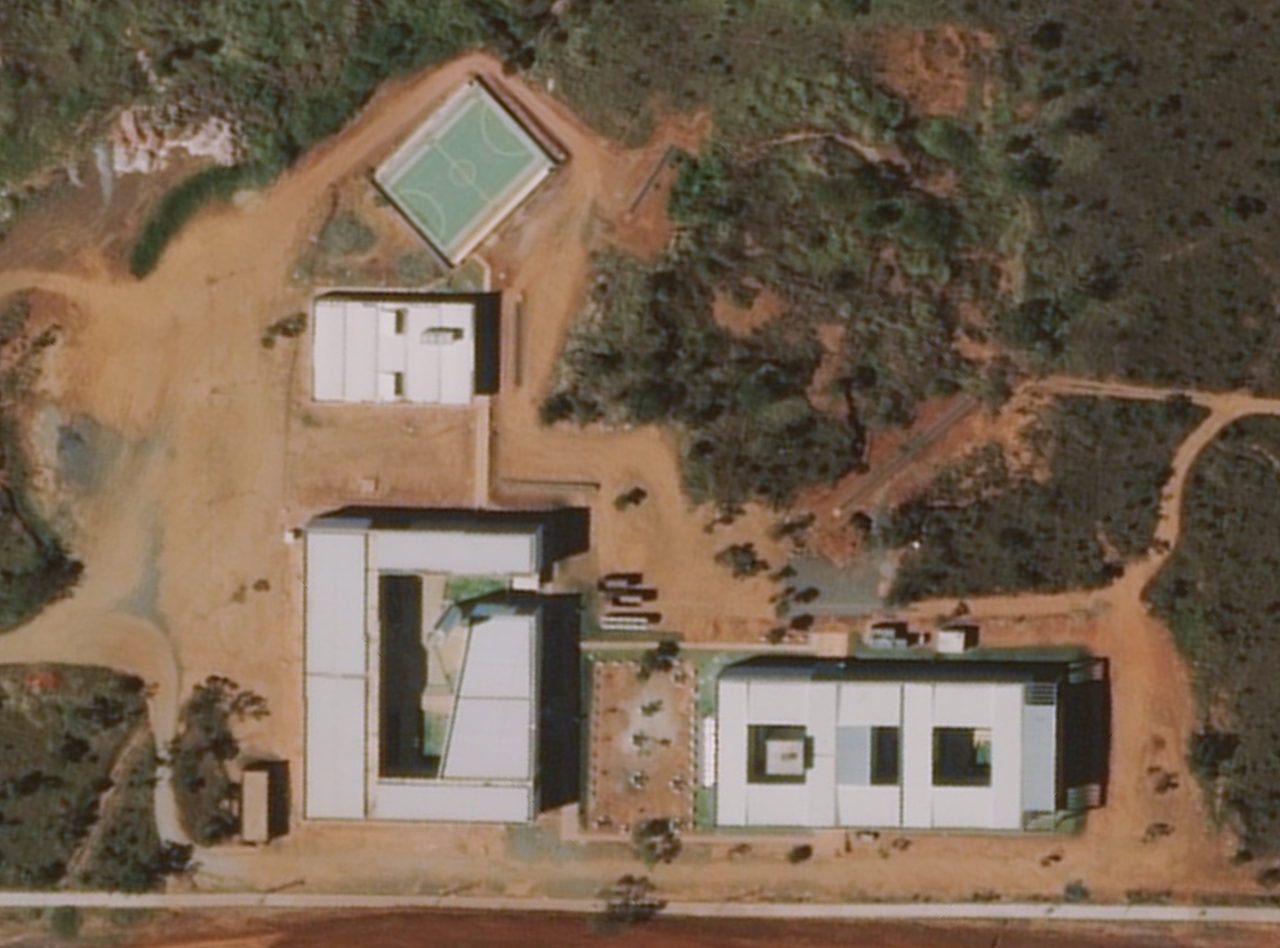
\includegraphics[width=0.6\textwidth]{figuras/fga1}
	\label{img:fga1}
\end{figure}

Dessa forma, foi elaborado um diagrama de espinha de peixe para avaliar os principais motivos pelos quais a comunidade da Faculdade do Gama sente-se insegura. Os problemas elencados apresentam estreita correlação com a falta de estrutura do campus e cercamento do local, ocasionando, por exemplo, a fuga rápida do indivíduo infrator. A falta de câmeras externas, a ausência de policiamento e a localização isolada do campus também facilitam ações criminosas. A espinha de peixe (\textit{fishbone}) pode ser observada na imagem \ref{img:fishbone}.

\begin{figure}[htp]
	\centering
	\caption{Principais motivos responsáveis pela falta de segurança no estacionamento do campus FGA.}
	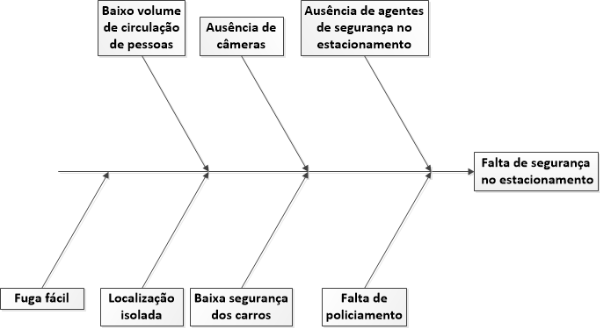
\includegraphics[width=0.6\textwidth]{figuras/fishbone}
	\label{img:fishbone}
\end{figure}

Também, como maneira de obter alguns dados referentes à mobilidade de alunos, professores e comunidade até o campus, o Grupo 1 da disciplina Projeto Integrador 1 decidiu aplicar uma pesquisa sobre o meio de transporte utilizado para deslocamento residência-campus, no qual foi perguntado quantas vezes o veículo foi roubado, se o indivíduo prestou alguma queixa formal (boletim de ocorrência) e o(s) ano(s) do ocorrido, caso este utilize automóvel para locomoção. O título da pesquisa pode ser observado na imagem. \ref{img:questionario}.

\begin{figure}[htp]
	\centering
	\caption{Questionário sobre mobilidade e segurança do campus.}
	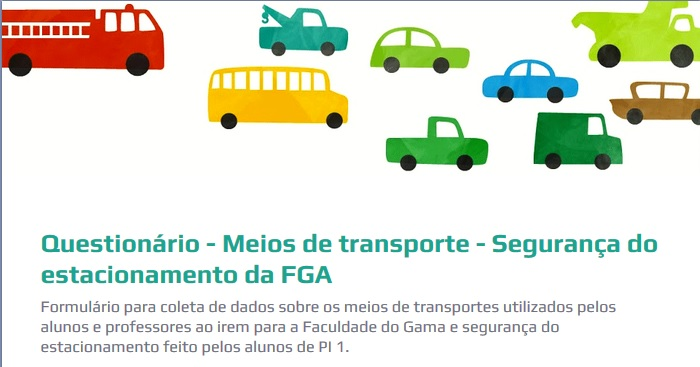
\includegraphics[width=0.6\textwidth]{figuras/questionario}
	\label{img:questionario}
\end{figure}

A pesquisa foi elaborada no aplicativo Google Drive - Formulários e publicada no período do dia 02 de agosto de 2015 ao dia 29 de agosto do mesmo ano no grupo destinado aos alunos e professores da UnB-Gama, na rede social Facebook. Durante este período, 93 pessoas responderam às seis questões propostas no questionário, resultando nos dados apresentados nos gráfico \ref{img:resultadoquestionario}.



Na quinta-feira anterior ao dia de apresentação do Ponto de Controle, o relatório preliminar deverá ser entregue ao professor orientador para uma revisão geral. Após as correções feitas pelos anos,  o relatório poderá  ser entregue via \textit{Moodle}.

\begin{table}[H]
\centering
\caption{Cronograma de atividades até o primeiro Ponto de Controle de PI 1.}
\begin{tabular}{|p{2.5cm}|p{0.5cm}|p{0.5cm}|p{0.5cm}|p{0.5cm}|p{0.5cm}|p{0.5cm}|p{0.5cm}|p{0.5cm}|p{0.5cm}|p{0.5cm}|p{0.5cm}|p{0.5cm}|p{0.5cm}|p{0.5cm}|p{0.5cm}|}
\hline
\multicolumn{16}{|c|}{Primeiro ponto de controle}                                                                                                                                                                                                                                                                                                                                                                          \\ \hline
Atividades                     & \scalebox{.7}{21/09}                     & \scalebox{.7}{22/09}                     & \scalebox{.7}{23/09}                     & \scalebox{.7}{24/09}                     & \scalebox{.7}{25/09}                     & \scalebox{.7}{26/09}                     & \scalebox{.7}{27/09}                     & \scalebox{.7}{28/09}                     & \scalebox{.7}{29/09}                     & \scalebox{.7}{30/09}                     & \scalebox{.7}{01/10}                     & \scalebox{.7}{02/10}                     & \scalebox{.7}{03/10} & \scalebox{.7}{04/10} & \scalebox{.7}{05/10}                     \\ \hline
Revisão bibliográfica          & \cellcolor{blue}X & \cellcolor{blue}X & \cellcolor{blue}X & \cellcolor{blue}X &                           &                           &                           &                           &                           &                           &                           &                           &       &       &                           \\ \hline
Definição escopo               &                           &                           &                           &                           & \cellcolor{blue}X &                           &                           &                           &                           &                           &                           &                           &       &       &                           \\ \hline
Revisão 1.0                    &                           &                           &                           &                           & \cellcolor{blue}X &                           &                           &                           &                           &                           &                           &                           &       &       &                           \\ \hline
Latex                          &                           &                           &                           &                           & \cellcolor{blue}X & \cellcolor{blue}X & \cellcolor{blue}X &                           &                           &                           &                           &                           &       &       &                           \\ \hline
Apresentação 1.0               &                           &                           &                           &                           &                           &                           &                           & \cellcolor{blue}X &                           &                           &                           &                           &       &       &                           \\ \hline
Revisão 2.0                    &                           &                           &                           &                           &                           &                           &                           & \cellcolor{blue}X & \cellcolor{blue}X & \cellcolor{blue}X & \cellcolor{blue}X &                           &       &       &                           \\ \hline
Revisão professor              &                           &                           &                           &                           &                           &                           &                           &                           &                           &                           & \cellcolor{blue}X & \cellcolor{blue}X &       &       &                           \\ \hline
Revisão 3.0                    &                           &                           &                           &                           &                           &                           &                           &                           &                           &                           &                           & \cellcolor{blue}X &       &       &                           \\ \hline
Apresentação ponto de controle &                           &                           &                           &                           &                           &                           &                           &                           &                           &                           &                           &                           &       &       & \cellcolor{blue}X \\ \hline
\end{tabular}
\label{tab:cronograma1}
\end{table}

\noindent \textbf{Legenda:} \\
\crule[blue]{0.5cm}{0.3cm}	Atividade realizada \\
\crule[red]{0.5cm}{0.3cm} Atividade não realizada \\

    \begin{table}[H]
    \centering
    \caption{Cronograma de atividades para o segundo  Ponto de Controle de PI 1.}
    \begin{tabular}{|p{2.5cm}|p{0.5cm}|p{0.5cm}|p{0.5cm}|p{0.5cm}|p{0.5cm}|p{0.5cm}|p{0.5cm}|p{0.5cm}|p{0.5cm}|p{0.5cm}|p{0.5cm}|p{0.5cm}|p{0.5cm}|p{0.5cm}|p{0.5cm}|}
    \hline
    \multicolumn{16}{|c|}{Segundo ponto de controle}                                                                                                                                                                                                                                                                                                                                                                                                                                                    \\ \hline
    Atividades                                                      & \scalebox{.7}{12/10}                     & \scalebox{.7}{13/10}                     & \scalebox{.7}{14/10}                     & \scalebox{.7}{15/10}                     & \scalebox{.7}{16/10}                     & \scalebox{.7}{17/10}                     & \scalebox{.7}{18/10}                     & \scalebox{.7}{19/10}                     & \scalebox{.7}{20/10}                     & \scalebox{.7}{21/10}                     & \scalebox{.7}{22/10}                     & \scalebox{.7}{23/10}                     & \scalebox{.7}{29/10}                     & \scalebox{.7}{30/10}                     & \scalebox{.7}{04/11}                     \\ \hline
    Revisão bibliográfica                                           & \cellcolor{blue}X & \cellcolor{blue}X & \cellcolor{blue}X & \cellcolor{blue}X &                           &                           &                           &                           &                           &                           &                           &                           &                           &                           &                           \\ \hline
    Aprimoramento de aspectos técnicos                              &                           &                           &                           & \cellcolor{blue}X & \cellcolor{blue}X & \cellcolor{blue}X &                           &                           &                           &                           &                           &                           &                           &                           &                           \\ \hline
    Elaboração de simulação Catia                                   &                           &                           & \cellcolor{blue}X & \cellcolor{blue}X & \cellcolor{blue}X & \cellcolor{blue}X & \cellcolor{blue}X & \cellcolor{blue}X &                           &                           &                           &                           &                           &                           &                           \\ \hline
    Qualidade das justificativa das escolhas (quadros comparativos) &                           &                           &                           &                           &                           &                           &                           &                           & \cellcolor{blue}X & \cellcolor{blue}X & \cellcolor{blue}X &                           &                           &                           &                           \\ \hline
    Revisão 1.0                                                     &                           &                           &                           &                           &                           &                           &                           &                           &                           &                           &                           & \cellcolor{blue}X &                           &                           &                           \\ \hline
    Revisão professor                                               &                           &                           &                           &                           &                           &                           &                           &                           &                           &                           &                           &                           & \cellcolor{blue}X &                           &                           \\ \hline
    Revisão 2.0                                                     &                           &                           &                           &                           &                           &                           &                           &                           &                           &                           &                           &                           & \cellcolor{blue}X & \cellcolor{blue}X &                           \\ \hline
    Apresentação ponto de controle                                  &                           &                           &                           &                           &                           &                           &                           &                           &                           &                           &                           &                           &                           &                           & \cellcolor{blue}X \\ \hline
    \end{tabular}
  \label{tab:cronograma2}
    \end{table}

\begin{table}[H]
\centering
\caption{Cronograma de atividades para o terceiro  Ponto de Controle de PI 1.}
  \begin{tabular}{|p{2.5cm}|p{0.5cm}|p{0.5cm}|p{0.5cm}|p{0.5cm}|p{0.5cm}|p{0.5cm}|p{0.5cm}|p{0.5cm}|p{0.5cm}|p{0.5cm}|p{0.5cm}|p{0.5cm}|p{0.5cm}|p{0.5cm}|p{0.5cm}|}
\hline
\multicolumn{16}{|c|}{Terceiro ponto de controle}                                                                                                                                                                                                                                                                                                                                                                 \\ \hline
Atividades            & \scalebox{.7}{11/11}                     & \scalebox{.7}{12/11}                     & \scalebox{.7}{13/11}                     & \scalebox{.7}{14/11}                     & \scalebox{.7}{15/11}                     & \scalebox{.7}{16/11}                     & \scalebox{.7}{17/11}                     & \scalebox{.7}{18/11}                     & \scalebox{.7}{19/11}                     & \scalebox{.7}{20/11}                     & \scalebox{.7}{21/11}                     & \scalebox{.7}{22/11} & \scalebox{.7}{25/11}                     & \scalebox{.7}{27/11} & \scalebox{.7}{30/11}                     \\ \hline
Revisão bibliográfica & \cellcolor{blue}X & \cellcolor{blue}X & \cellcolor{blue}X & \cellcolor{blue}X &                           &                           &                           &                           &                           &                           &                           &       &                           &       &                           \\ \hline
Relação de custo      &                           &                           &                           & \cellcolor{blue}X & \cellcolor{blue}X & \cellcolor{blue}X &                           &                           &                           &                           &                           &       &                           &       &                           \\ \hline
Viabilidade econômica &                           &                           &                           &                           &                           & \cellcolor{blue}X & \cellcolor{blue}X & \cellcolor{blue}X & \cellcolor{blue}X &                           &                           &       &                           &       &                           \\ \hline
Revisão               &                           &                           &                           &                           &                           &                           &                           &                           &                           & \cellcolor{blue}X & \cellcolor{blue}X &       &                           &       &                           \\ \hline
Revisão professor     &                           &                           &                           &                           &                           &                           &                           &                           &                           &                           &                           &       & \cellcolor{blue}X &       &                           \\ \hline
Revisão final         &                           &                           &                           &                           &                           &                           &                           &                           &                           &                           &                           &       &                           &       & \cellcolor{blue}X \\ \hline
Apresentação final    &                           &                           &                           &                           &                           &                           &                           &                           &                           &                           &                           &       &                           &       & \cellcolor{blue}X \\ \hline
\end{tabular}
  \label{tab:cronograma3}
\end{table}
